% !TeX root = ../DistributedConsensus.tex
% !TeX spellcheck = en_GB
\chapter{Reducing Histories to Order of Execution}
\label{chap:order-of-execution}
\section{Order of Execution}
	When a combined history has been produced, it represents every action that has occurred on an event in the workflow. 
	Only an order of execution is desired and excess information in the history therefore needs to be reduced in order to only find execution information. 
	
	\subsection{Collapsing}
	Although the receiver saves incoming actions, these actions are still initiated by the performer, and these actions can therefore be seen as being parts of the performers execution. 
		
	It is necessary to determine what should represent the time of an execution. Possible candidates would be \texttt{ExecuteFinish} and \texttt{ExecuteStart}. Using \texttt{ExecuteFinish}, it is difficult to tell which execution happened before the other, due to the fact that actions that are part of an execution happen before the \texttt{ExecuteFinish} action. 
	The same applies for the \texttt{ExecuteStart} action, where actions that are part of an execution can happen after the execution.
	
	\newpar It then is necessary to research a way to \textit{collapse} an execution in order to overcome these problems. \textit{Collapsing} constitutes looking at all actions between an \texttt{ExecuteStart} action and an \texttt{ExecuteFinish} action of an event and connecting these events into a single entity, representing an entire execution. 
	
	Actions between start and finish might contain relations to other actions located in the local histories of other events. Since a given event is only affected by the effects of other events executing, it is safe to collapse the incoming actions from executing events into execution of the executing event. Since an action is always caused by the execution of \textit{some} event, the collapsed execution has the property that no action can happened outside any collapsed execution.
	
	An example of this separation of executions can be found in \autoref{fig:validation:collapsing}.
	
	\begin{figure}[H]
		\centering
		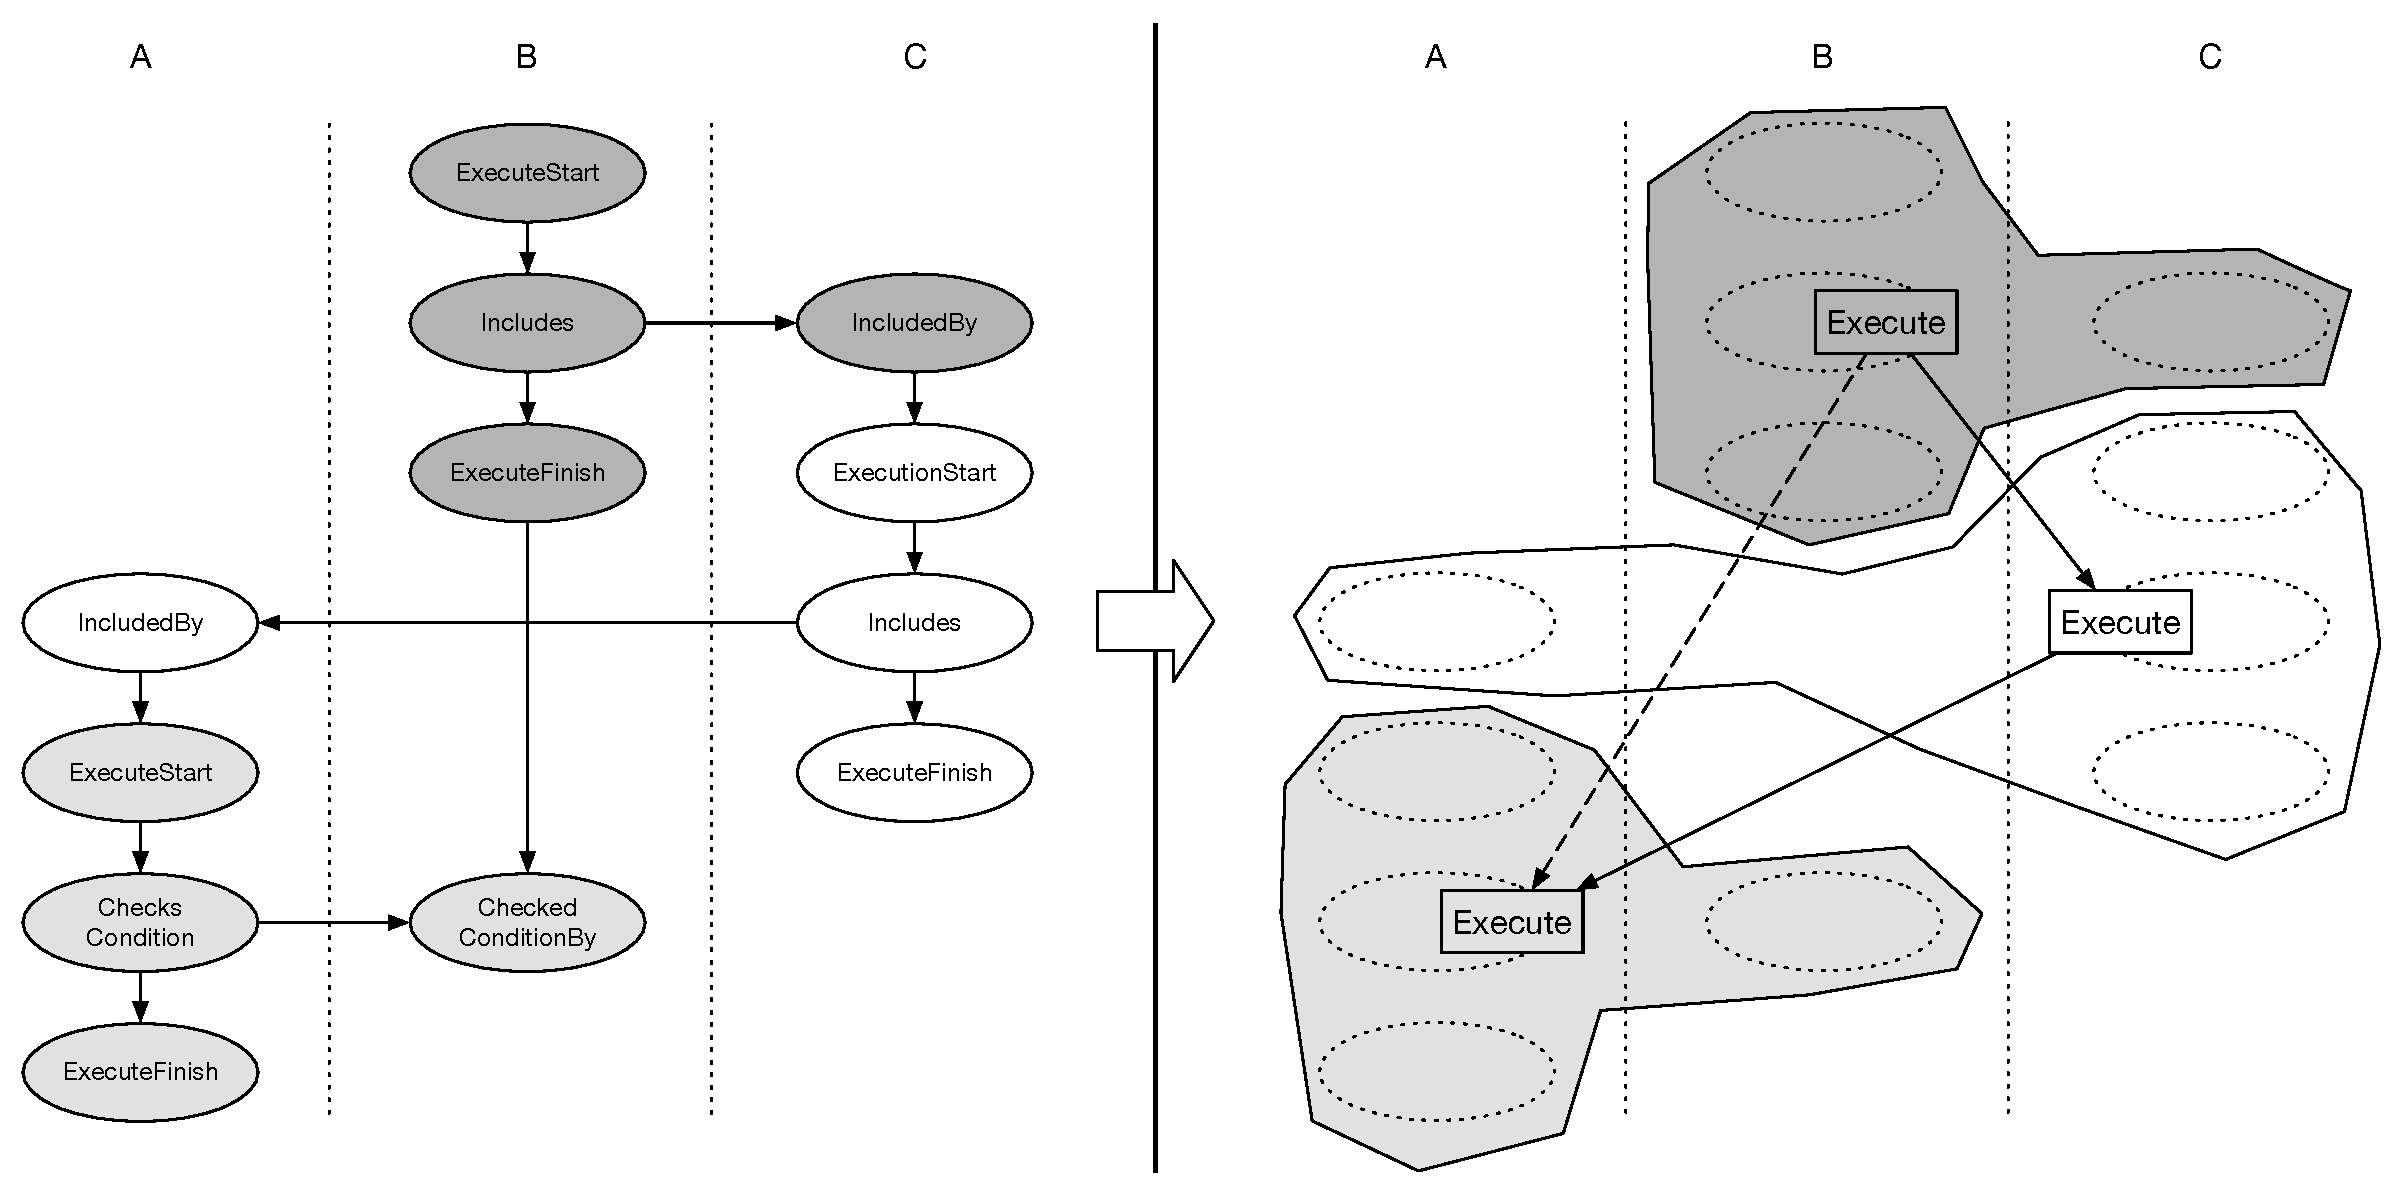
\includegraphics[width=\textwidth]{6orderofexecution/images/transitive-reduction-collapse.pdf}
		\caption{The result of collapsing actions in the histories of three events.}
		\label{fig:validation:collapsing}
	\end{figure}
	
	\begin{figure}
		\centering
		\def\svgwidth{0.42\columnwidth}
		\fontsize{6}{8}\selectfont
		\import{4connect/images/}{before_collapsing.pdf_tex}
		\caption{Separation of executions}
		\label{fig:before-collapsing}
	\end{figure}
	\todo{Denne figur skal laves ud fra GasWorkflow.}
	
	\newpar When actions contained in an execution have been found, it is necessary to decide what should happen to the grouping of the actions. It is desired to keep all relations intact, to avoid modifying the history and only simplify it. 
	
	By pointing all ingoing edges to the current event towards a new \textit{collapsed node}, and adding all outgoing edges to the new node, this is accomplished. This new \textit{collapsed node} then represents the entire execution. 
	
	In the implemented solution the the \texttt{ExecuteFinish} type has been chosen to denote a collapsed execution in order to avoid creating a new action type. As it can be seen in \autoref{fig:after-collapsing} the collapsing of executions results in an order of execution.
	\todo{udvid (find bedre eksempel) med at særlige tilfælde kræver transitive reduction efter\-følgende}
	
	\begin{figure}
		\centering
		\def\svgwidth{0.22\columnwidth}
		\fontsize{6}{8}\selectfont
		\import{4connect/images/}{after_collapsing.pdf_tex}
		\caption{Executions after collapsing}
		\label{fig:after-collapsing}
	\end{figure}
	\todo{Denne figur skal laves ud fra GasWorkflow.}
	
	The Collapse algorithm can be seen in \autoref{alg:collapse}.
	
	\begin{algorithm}
		\begin{algorithmic}
			\Function{Collapse}{graph}\State
				locals: CollapseMap: Mapping from old to newaction IDs.
				\State\hspace{28pt} Result: Graph, initially empty
				\State
				\State ExecuteStarts $\leftarrow$ \Call{Filter}{type = ExecuteStart, graph} \State
				Executions $\leftarrow$ \Call{Map.map}{FindSingleExecution, ExecuteStarts}
				\ForAll{executions in Executions}\State
					CollapseMap $\leftarrow$ \Call{CreateExecutionMap}{execution, newExecutionId, CollapseMap}
				\EndFor
				\ForAll{oldActionID, newActionID in CollapseMap}
					\State
					NewAction $\leftarrow$ Action with \State\hspace{28pt}ID = newActionID and \State\hspace{28pt}Edges = edges from oldActionID in graph mapped to new IDs\State
					Result $\leftarrow$ \Call{AddNode}{NewAction, Result} \State\Comment{This requires AddNode to merge edge sets when existing nodes are added}
				\EndFor
				
			\EndFunction
			\State
			\Function{FindSingleExecution}{startAction}
				\State locals: execution
				\While{startAction.Type $\neq$ ExecuteFinish} \State
					execution $\leftarrow$ \Call{AddRange}{startAction.Edges, execution}
				\EndWhile\State
				\Return execution
			\EndFunction
			\State
			\Function{CreateExecutionMap}{ActionSet, newActionId, accumulatorMap}
				\ForAll{actions in ActionSet}\State
					accumulatorMap $\leftarrow$ \Call{Add}{action.Id, newActionId, accumulatorMap}
				\EndFor \State
				\Return accumulatorMap
			\EndFunction
		\end{algorithmic}
		\caption{Collapse algorithm}
		\label{alg:collapse}
	\end{algorithm}
	
%    \subsection{Correctnes}
	The found order of execution still represents the same history and have the same properties as to the order. Given the definition of serially equivalence, which executions complies with, two processes happen after one another. Therefore the set of actions which are after actions in an execution must happen after that execution finishes, just as well as all action which happen before actions in an execution must happen before the execution starts. 

    
	\subsection{Transitive Reduction}
	
	\newpar Redundant edges might still exist in the history after the executions of the history have been collapsed. 
	In cases where a path from an action to another action as well as a direct edge between the two exists, the direct edge is redundant and can be removed. 
	
	\newpar Recall that a subgraph of the history with the same ordering and reachability, but as few edges as possible, is a \textit{minimum equivalent graph}. If there is a path from an edge $x$ to an edge $y$ in graph G, there must also be a path from $x$ to $y$ in the transitive reduction of $G$, and vice versa. 
	
	The minimum equivalent graph of the order of execution is desired, in order to remove redundant edges. 
	
	It is possible to find the minimum equivalent graph by transitive reduction of the collapsed graph, which results in the desired subgraph containing no redundant edges.
	
	\begin{algorithm}
		\begin{algorithmic}
			\Function{Execution Transitive-Reduction}{history}
				\ForAll{action1 in history}
					\ForAll{action2 in history}
						\If{\Call{pathExists}{action1, action2, history}}
							\ForAll{action3 in history}
								\If{\Call{edgeExists}{action2, action3, history}}
									\If{\Call{edgeExists}{action1, action3, history}}
										\State history $\leftarrow$ \Call{removeEdge} {action1, action3, history}
									\EndIf
								\EndIf
							\EndFor
						\EndIf
					\EndFor
				\EndFor
			\State
			\Return history
			\EndFunction
		\end{algorithmic}
		\caption{Transitive Reduction Algorithm}
	\end{algorithm}
	\todo[inline]{Fjern algoritme?}
	
	\newpar The implemented algorithm for transitive reduction runs in $O(n^3)$ where $n$ is the number of actions, due to the fact that the algorithm has three nested for-loops over all actions in the history. This is based on the requirements that $pathExist$ runs in linear time and $edgeExist$ is a constant lookup. In actual use cases the graph will not be totally connected and therefore the innermost loop will not be executed for most actions.
	
	\newpar By combining these two collapsing and reduction steps, the order of execution represented as a minimum equivalent graph of the entire history is found. 
	
	\newpar These algorithms do not provide a way to ensure that malicious nodes cannot falsify the history. As in the case where one event represented the workflow, there is no way of making sure that the event creating the history will not tamper with the history. It would be possible to pinpoint which neighbouring events are malicious if enough of the neighbours have relations to each other. 

	\section{Election} 
	As we have now found an order of execution where (potentially) malicious events have been identified, we want to know if the remaining events can agree upon the rest of order of execution.
	
	\newpar As stated in the problem definition, it is desired to reach consensus on the resulting order of execution, but since no process in the system knows the entire state of a workflow, it is not possible for the events to suggest an order of execution without completing steps alike with the ones described in this report.
	
	\newpar Because we have chosen to let the client know all events in order to retrieve their histories, it is also easy for us to send the resulting order of execution back to them, in order to find out whether or not they can agree to this order.
	
	\newpar When any event receives this order of execution, it can look at its own history and at the received order. In a good event the local history can contain executions with outgoing actions between execute start and execute finish actions. Furthermore ingoing relations can be identified as executions of other events from the following rules:
	
	\begin{itemize}
		\item Each counterpart present in actions with ingoing action types must have executed at least once, in order to contact the local event.
		\item If two actions with the same ingoing action type and counterpart are present after each other, this denotes two separate executions of the counterpart event, because each executing event only contacts another event once per relation when executing.
	\end{itemize}
	
	\newpar Furthermore if an event has sent multiple ingoing requests as part of a single execution, then each of the relations that these actions represent must be present every time that execution has happened. Given these rules, the local history can be turned into a "local order of execution".
	
	\newpar In order for the event to agree on the global order of execution, if there exists a path from one execution to another in the local order of execution, there must also exist a path between these executions in the global order of execution.
	
	\newpar \todo[inline]{Hvordan bruger vi det her til at skrive at election i virkeligheden er en bekræftelse af vores algoritme, mere end det er en egentlig afstemning om resultatet?}